\chapter{The Challenge}

Then,” continued Beauchamp, “I took advantage of the silence and the
darkness to leave the house without being seen. The usher who had
introduced me was waiting for me at the door, and he conducted me
through the corridors to a private entrance opening into the Rue de
Vaugirard. I left with mingled feelings of sorrow and delight. Excuse
me, Albert,—sorrow on your account, and delight with that noble girl,
thus pursuing paternal vengeance. Yes, Albert, from whatever source the
blow may have proceeded—it may be from an enemy, but that enemy is only
the agent of Providence.”

Albert held his head between his hands; he raised his face, red with
shame and bathed in tears, and seizing Beauchamp’s arm:

“My friend,” said he, “my life is ended. I cannot calmly say with you,
‘Providence has struck the blow;’ but I must discover who pursues me
with this hatred, and when I have found him I shall kill him, or he
will kill me. I rely on your friendship to assist me, Beauchamp, if
contempt has not banished it from your heart.”

“Contempt, my friend? How does this misfortune affect you? No, happily
that unjust prejudice is forgotten which made the son responsible for
the father’s actions. Review your life, Albert; although it is only
just beginning, did a lovely summer’s day ever dawn with greater purity
than has marked the commencement of your career? No, Albert, take my
advice. You are young and rich—leave Paris—all is soon forgotten in
this great Babylon of excitement and changing tastes. You will return
after three or four years with a Russian princess for a bride, and no
one will think more of what occurred yesterday than if it had happened
sixteen years ago.”

“Thank you, my dear Beauchamp, thank you for the excellent feeling
which prompts your advice; but it cannot be. I have told you my wish,
or rather my determination. You understand that, interested as I am in
this affair, I cannot see it in the same light as you do. What appears
to you to emanate from a celestial source, seems to me to proceed from
one far less pure. Providence appears to me to have no share in this
affair; and happily so, for instead of the invisible, impalpable agent
of celestial rewards and punishments, I shall find one both palpable
and visible, on whom I shall revenge myself, I assure you, for all I
have suffered during the last month. Now, I repeat, Beauchamp, I wish
to return to human and material existence, and if you are still the
friend you profess to be, help me to discover the hand that struck the
blow.”

“Be it so,” said Beauchamp; “if you must have me descend to earth, I
submit; and if you will seek your enemy, I will assist you, and I will
engage to find him, my honor being almost as deeply interested as
yours.”

“Well, then, you understand, Beauchamp, that we begin our search
immediately. Each moment’s delay is an eternity for me. The calumniator
is not yet punished, and he may hope that he will not be; but, on my
honor, if he thinks so, he deceives himself.”

“Well, listen, Morcerf.”

“Ah, Beauchamp, I see you know something already; you will restore me
to life.”

“I do not say there is any truth in what I am going to tell you, but it
is, at least, a ray of light in a dark night; by following it we may,
perhaps, discover something more certain.”

“Tell me; satisfy my impatience.”

“Well, I will tell you what I did not like to mention on my return from
Yanina.”

“Say on.”

“I went, of course, to the chief banker of the town to make inquiries.
At the first word, before I had even mentioned your father’s name”—

“‘Ah,’ said he. ‘I guess what brings you here.’

“‘How, and why?’

“‘Because a fortnight since I was questioned on the same subject.’

“‘By whom?’

“‘By a banker of Paris, my correspondent.’

“‘Whose name is——’

“‘Danglars.’”

“He!” cried Albert; “yes, it is indeed he who has so long pursued my
father with jealous hatred. He, the man who would be popular, cannot
forgive the Count of Morcerf for being created a peer; and this
marriage broken off without a reason being assigned—yes, it is all from
the same cause.”

“Make inquiries, Albert, but do not be angry without reason; make
inquiries, and if it be true——”

“Oh, yes, if it be true,” cried the young man, “he shall pay me all I
have suffered.”

“Beware, Morcerf, he is already an old man.”

“I will respect his age as he has respected the honor of my family; if
my father had offended him, why did he not attack him personally? Oh,
no, he was afraid to encounter him face to face.”

“I do not condemn you, Albert; I only restrain you. Act prudently.”

“Oh, do not fear; besides, you will accompany me. Beauchamp, solemn
transactions should be sanctioned by a witness. Before this day closes,
if M. Danglars is guilty, he shall cease to live, or I shall die.
\textit{Pardieu}, Beauchamp, mine shall be a splendid funeral!”

“When such resolutions are made, Albert, they should be promptly
executed. Do you wish to go to M. Danglars? Let us go immediately.”

They sent for a cabriolet. On entering the banker’s mansion, they
perceived the phaeton and servant of M. Andrea Cavalcanti.

“Ah! \textit{parbleu!} that’s good,” said Albert, with a gloomy tone. “If M.
Danglars will not fight with me, I will kill his son-in-law; Cavalcanti
will certainly fight.”

The servant announced the young man; but the banker, recollecting what
had transpired the day before, did not wish him admitted. It was,
however, too late; Albert had followed the footman, and, hearing the
order given, forced the door open, and followed by Beauchamp found
himself in the banker’s study.

“Sir,” cried the latter, “am I no longer at liberty to receive whom I
choose in my house? You appear to forget yourself sadly.”

“No, sir,” said Albert, coldly; “there are circumstances in which one
cannot, except through cowardice,—I offer you that refuge,—refuse to
admit certain persons at least.”

“What is your errand, then, with me, sir?”

“I mean,” said Albert, drawing near, and without apparently noticing
Cavalcanti, who stood with his back towards the fireplace—“I mean to
propose a meeting in some retired corner where no one will interrupt us
for ten minutes; that will be sufficient—where two men having met, one
of them will remain on the ground.”

Danglars turned pale; Cavalcanti moved a step forward, and Albert
turned towards him.

“And you, too,” said he, “come, if you like, monsieur; you have a
claim, being almost one of the family, and I will give as many
rendezvous of that kind as I can find persons willing to accept them.”

Cavalcanti looked at Danglars with a stupefied air, and the latter,
making an effort, arose and stepped between the two young men. Albert’s
attack on Andrea had placed him on a different footing, and he hoped
this visit had another cause than that he had at first supposed.

“Indeed, sir,” said he to Albert, “if you are come to quarrel with this
gentleman because I have preferred him to you, I shall resign the case
to the king’s attorney.”

“You mistake, sir,” said Morcerf with a gloomy smile; “I am not
referring in the least to matrimony, and I only addressed myself to M.
Cavalcanti because he appeared disposed to interfere between us. In one
respect you are right, for I am ready to quarrel with everyone today;
but you have the first claim, M. Danglars.”

\begin{figure}[ht]
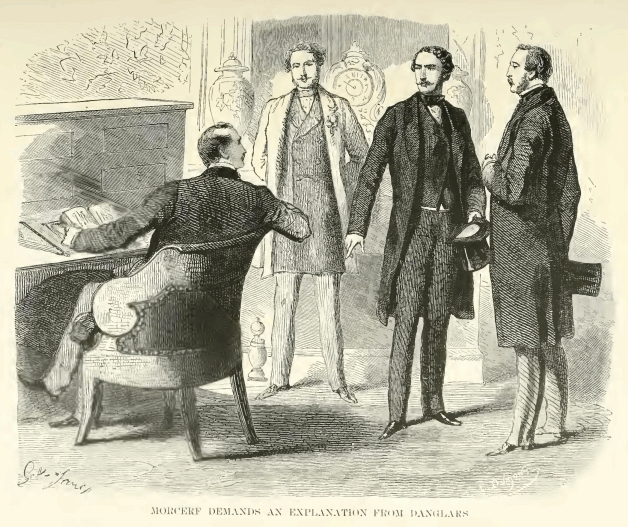
\includegraphics[width=\textwidth]{40212m.jpg}
\end{figure}

“Sir,” replied Danglars, pale with anger and fear, “I warn you, when I
have the misfortune to meet with a mad dog, I kill it; and far from
thinking myself guilty of a crime, I believe I do society a kindness.
Now, if you are mad and try to bite me, I will kill you without pity.
Is it my fault that your father has dishonored himself?”

“Yes, miserable wretch!” cried Morcerf, “it is your fault.”

Danglars retreated a few steps. “My fault?” said he; “you must be mad!
What do I know of the Grecian affair? Have I travelled in that country?
Did I advise your father to sell the castle of Yanina—to betray——”

“Silence!” said Albert, with a thundering voice. “No; it is not you who
have directly made this exposure and brought this sorrow on us, but you
hypocritically provoked it.”

“I?”

“Yes; you! How came it known?”

“I suppose you read it in the paper in the account from Yanina?”

“Who wrote to Yanina?”

“To Yanina?”

“Yes. Who wrote for particulars concerning my father?”

“I imagine anyone may write to Yanina.”

“But one person only wrote!”

“One only?”

“Yes; and that was you!”

“I, doubtless, wrote. It appears to me that when about to marry your
daughter to a young man, it is right to make some inquiries respecting
his family; it is not only a right, but a duty.”

“You wrote, sir, knowing what answer you would receive.”

“I, indeed? I assure you,” cried Danglars, with a confidence and
security proceeding less from fear than from the interest he really
felt for the young man, “I solemnly declare to you, that I should never
have thought of writing to Yanina, did I know anything of Ali Pasha’s
misfortunes.”

“Who, then, urged you to write? Tell me.”

“\textit{Pardieu!} it was the most simple thing in the world. I was speaking
of your father’s past history. I said the origin of his fortune
remained obscure. The person to whom I addressed my scruples asked me
where your father had acquired his property? I answered, ‘In
Greece.’—‘Then,’ said he, ‘write to Yanina.’”

“And who thus advised you?”

“No other than your friend, Monte Cristo.”

“The Count of Monte Cristo told you to write to Yanina?”

“Yes; and I wrote, and will show you my correspondence, if you like.”

Albert and Beauchamp looked at each other.

“Sir,” said Beauchamp, who had not yet spoken, “you appear to accuse
the count, who is absent from Paris at this moment, and cannot justify
himself.”

“I accuse no one, sir,” said Danglars; “I relate, and I will repeat
before the count what I have said to you.”

“Does the count know what answer you received?”

“Yes; I showed it to him.”

“Did he know my father’s Christian name was Fernand, and his family
name Mondego?”

“Yes, I had told him that long since, and I did only what any other
would have done in my circumstances, and perhaps less. When, the day
after the arrival of this answer, your father came by the advice of
Monte Cristo to ask my daughter’s hand for you, I decidedly refused
him, but without any explanation or exposure. In short, why should I
have any more to do with the affair? How did the honor or disgrace of
M. de Morcerf affect me? It neither increased nor decreased my income.”

Albert felt the blood mounting to his brow; there was no doubt upon the
subject. Danglars defended himself with the baseness, but at the same
time with the assurance, of a man who speaks the truth, at least in
part, if not wholly—not for conscience’ sake, but through fear.
Besides, what was Morcerf seeking? It was not whether Danglars or Monte
Cristo was more or less guilty; it was a man who would answer for the
offence, whether trifling or serious; it was a man who would fight, and
it was evident Danglars would not fight.

In addition to this, everything forgotten or unperceived before
presented itself now to his recollection. Monte Cristo knew everything,
as he had bought the daughter of Ali Pasha; and, knowing everything, he
had advised Danglars to write to Yanina. The answer known, he had
yielded to Albert’s wish to be introduced to Haydée, and allowed the
conversation to turn on the death of Ali, and had not opposed Haydée’s
recital (but having, doubtless, warned the young girl, in the few
Romaic words he spoke to her, not to implicate Morcerf’s father).
Besides, had he not begged of Morcerf not to mention his father’s name
before Haydée? Lastly, he had taken Albert to Normandy when he knew the
final blow was near. There could be no doubt that all had been
calculated and previously arranged; Monte Cristo then was in league
with his father’s enemies. Albert took Beauchamp aside, and
communicated these ideas to him.

“You are right,” said the latter; “M. Danglars has only been a
secondary agent in this sad affair, and it is of M. de Monte Cristo
that you must demand an explanation.”

Albert turned.

“Sir,” said he to Danglars, “understand that I do not take a final
leave of you; I must ascertain if your insinuations are just, and am
going now to inquire of the Count of Monte Cristo.”

He bowed to the banker, and went out with Beauchamp, without appearing
to notice Cavalcanti. Danglars accompanied him to the door, where he
again assured Albert that no motive of personal hatred had influenced
him against the Count of Morcerf.
